%!TEX root = ../Thesis.tex

\chapter{Untersuchung verschiedener Straßentopologien}
\label{cha:street_topologies}

% Beschreibung möglicher (Auswahl) Straßentopologien und ihrer Herausforderungen für die Erkennung von Fahrbahnen
% Idealerweise immer Bild einer entsprechenden Topologie und der entsprechenden Roh-Trajektorien
% Erläuterung: Was ist eine "Fahrspur" in dieser Arbeit. (d.h. nicht notwendigerweise eine Spur, wie sie auf Straße markiert ist.
% Beschreibt übliche Fahrbahn eines Fahrzeugs?!)

In diesem Kapitel werden wichtige und häufig vorkommende Straßentopologien vorgestellt.
Es wird untersucht, welche Herausforderungen bei der Erkennung von Fahrspuren im Fall der unterschiedlichen
Topologien existieren.

% Landstraßen (ein / zweispurig),
\section{``Normale'' Straßenabschnitte}

Mit ``normalen'' Straßenabschnitten sind hier all jene gemeint, welche keine Kreuzung, keinen Kreisverkehr
oder ähnliches beinhalten. Mehrere Fahrspuren in einem solchen Abschnitt verlaufen parallel zueinander
und sind üblicherweise klar getrennt.
Häufig zu finden sind ``normale'' Straßenabschnitte auf Landstraßen oder Autobahnen. In Abbildung
\ref{fig:topos_normal_lanes} sind zwei Beispiele normaler Straßenabschnitte dargestellt.

% TODO: 
\begin{figure}[H]
    \centering
    \subfloat[Landstraße]{{
        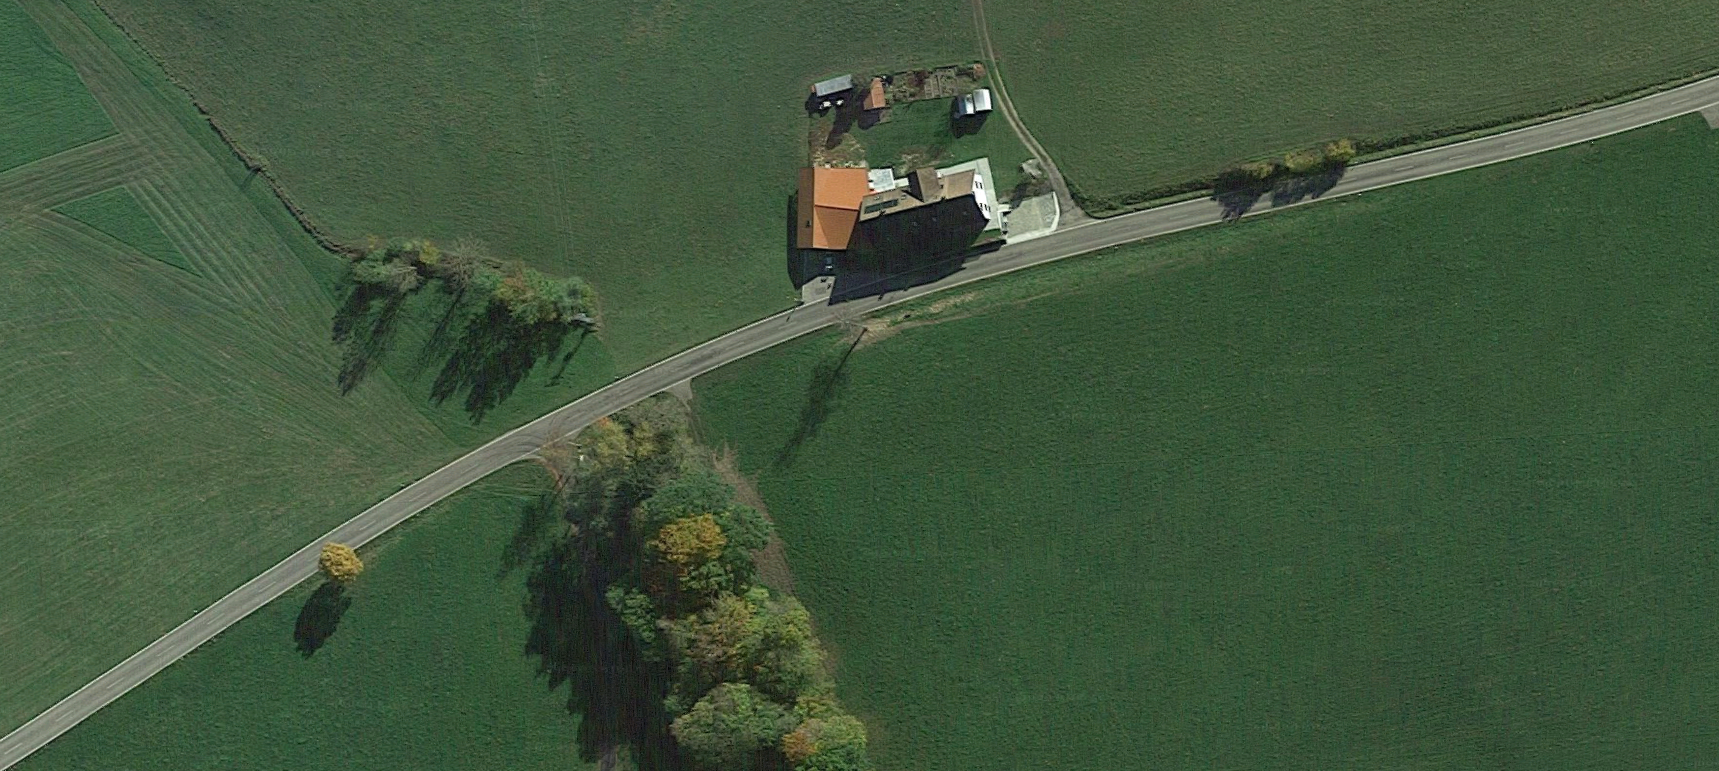
\includegraphics[align=c, width=0.40\linewidth]{resources/img/topos/landstrasse_1}
    }}
    \qquad \qquad
    \subfloat[Autobahn]{{
        \includegraphics[align=c, width=0.34\linewidth]{resources/img/topos/Autobahn}
    }}
    \caption{Beispiele normaler Straßenabschnitte}
    \label{fig:topos_normal_lanes}
\end{figure}

Unterschieden werden muss zwischen Fahrbahnen mit nur einer oder mit mehreren Fahrspuren. Besitzt
eine Fahrbahn nur eine Fahrspur und es handelt sich bei ihr nicht um eine Einbahnstraße, so bewegen
sich Fahrzeuge auf dieser Spur in beide Richtungen. Dies erschwert die Bestimmung der Fahrspuren,
da die Trajektorien der Fahrzeuge auf einer Spur in entgegengesetzte Richtungen verlaufen.
In einer solchen Situation zwei disjunkte Spuren zu identifizieren ist nicht immer möglich.
Ansonsten ist die Erkennung von Fahrspuren im Fall dieser Topologien allerdings verhältnismäßig unkompliziert,
da die Bewegungsbahnen der Fahrzeuge in der Regel gut in Cluster unterteilt werden können und keine Überlagerungen
von Spuren existieren.

% Kreuzungen (inkl. Abbiegespuren)
\section{Kreuzungen}

% Fahrbahnen kreuzen sich, geregelt über Ampelanlagen oder Rechts-vor-Links
% Abbiegespuren
% Fahrspuren überlagern sich. Sinnvolle Aufteilung

Kreuzungen stellen eine etwas kompliziertere Straßentopologie dar. Die in einem Streckenabschnitt mit
Kreuzung enthaltenen Fahrspuren verlaufen nicht alle parallel zueinander sondern überlagern sich
Abschnittsweise.

\begin{figure}[H]
\centering
    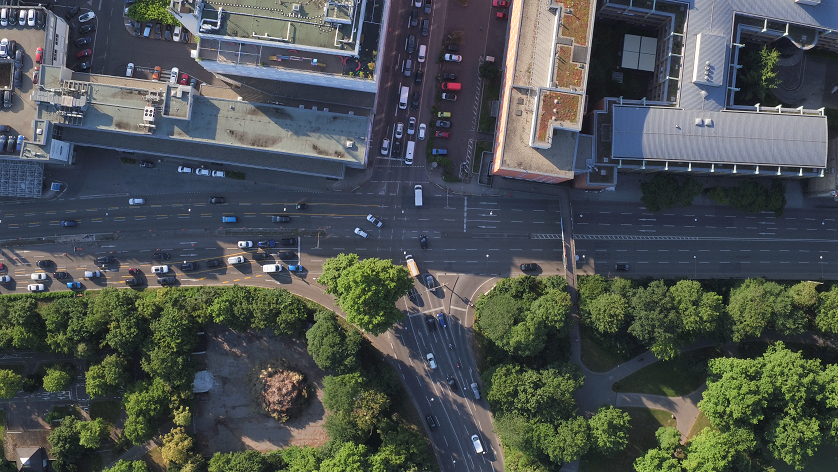
\includegraphics[width=0.5\linewidth]{resources/img/umsetzung/U1/Neckartor_Aufnahme}
\caption{Beispiel Kreuzung}
\label{fig:topos_crossroad}
\end{figure}

% Kreisverkehre
\section{Kreisverkehre}

% 12 Bewegungsbahnen durch Kreisverkehr (ausgenommen 360Grad Wendungen etc.)
% schwierig zu definieren, wie fahrspuren durch Kreisverkehr verlaufen
% Welche partitionieren
% Werden alle Bahnen richtig erkannt? Viele Überdeckungen. Richtig geclusterd?

\section{Sich öffnende oder schließende Fahrspuren}